\documentclass[a4paper,english]{article}
\usepackage[T1]{fontenc}
\usepackage[latin9]{inputenc}
\usepackage{float}
\usepackage{graphicx}
\usepackage{hyperref}
\graphicspath{{figures/}{../source/}}

\usepackage{babel}
\begin{document}
\title{The Method of Artificial Systems}
\author{Christopher A. Tucker\\
\small \texttt{cartheur@pm.me}\\
\small \href{https://orcid.org/0000-0002-0172-7258}{ORCID: 0000-0002-0172-7258}}
\date{}
\maketitle
\begin{abstract}
Artificial life is embodied AI. It becomes buildable when hardware
and software are tightly coupled, behavior is kept compact, process
is asynchronous and local, memory is held within nodes, communication
is explicit, and experiment remains reproducible at the board level.
Under those conditions, synthetic systems can be studied as situated,
adaptive forms of machine life. Here, it is grounded in the Volatco
board experiments as a repeatable demonstration in behavior, coordination,
energy, and adaptation.
\end{abstract}

\section{Preface}

Artificial life is embodied AI. By applying a few architectural rules,
including tight coupling between hardware and software, compact behavior
representations, asynchronous local process, in-node memory words,
explicit communication, and reproducible board-level experiment, something
living becomes buildable.

Related works by the same author pursue narrower parts of that program.
Historical and conceptual lineage is developed elsewhere through studies
of symbolic logic, machine control, embodied intelligence, code-level
robotic behavior, and substrate-oriented architecture. Those adjacent
works matter here only because they show that the method of artificial
systems is not a detached philosophical stance, but part of a constructive
research line.

What matters here is method: the vocabulary, design principles, and
experimental orientation needed to treat synthetic entities as situated
systems rather than as incomplete copies of human intelligence.

The proof path is distributed across the companion papers. The symbolic-logic
study recovers the architectural claim that sensing, state, control,
action, and adaptation belong to one machine-intelligence design problem.
Behavior diagrams extract a compact behavioral vocabulary from preserved
robot software. The hybrid-substrate study carries that
vocabulary toward execution through node-local process, asynchronous
communication, boot-time initialization, and functional simulation.
Together with the Volatco board experiments, those works are used here
to demonstrate that artificial life is embodied AI, where reset conditions, pin maps,
watchdog behavior, message handoff, power draw, and pass/fail criteria
can be made explicit and repeated.

The methodological consequence is direct. Artificial systems become
more intelligible, more designable, and more experimentally productive
when they are treated as living technical entities rather than as
incomplete imitations of the human mind. The strongest current output
of that formulation is not a generalized robot mythology, but a reproducible
board experiment in which behavior, coordination, energy, and adaptation
can be tested under ordinary scientific conditions.


\section{Introduction}

The question guiding this work is not merely whether machines can
be called intelligent. It is whether the dominant conceptual frame
for artificial intelligence has also limited our ability to build
and understand artificial forms of life. Much of the language surrounding
AI encourages researchers to judge machines by how closely they resemble
selective features of human cognition. That orientation has produced
useful tools, but it has also narrowed the design space. It encourages
imitation where a more fruitful path may be construction.

This manuscript takes a different position. Machines should not be
designed primarily as reduced copies of human intelligence, nor should
they be forced into conceptual models whose assumptions do not fit
the systems being built. They should instead be approached as artificial
systems: organized entities with their own constraints, behaviors,
relations to environments, and modes of adaptation. Under this view,
the task is not to ask whether a machine
imperfectly resembles a person, but to determine what kinds of autonomy,
coordination, and situated choice can be engineered into a synthetic
entity and how those capacities can be studied rigorously.

The argument developed here is that artificial life requires a design
methodology centered on context, orchestration, and choice. Context
matters because no adaptive system can be understood apart from the
conditions in which it acts. Orchestration matters because complex
behavior depends on the coordination of heterogeneous physical and
abstract components. Choice matters because adaptation requires more
than reaction; it requires structured discretionary limits within
which an entity can generate behavior that is neither wholly fixed
nor wholly arbitrary. These three ideas form the core of the method
proposed in this work.

The sibling hybrid-substrate paper sharpens this further by giving those
ideas an implementation grammar. In that paper, behavior does not remain
an interpretive diagram. It is treated as something assignable to local
nodes, carried by explicit ports, stabilized by node-local memory, and
made reproducible through declarative initialization. That execution
story is the strongest present proof that the method proposed here can
be realized as embodied artificial life rather than left at the level
of terminology.

This project has three linked aims. First, it defines a conceptual
vocabulary adequate to the design of synthetic entities. Second, it
proposes a methodological framework for organizing the features, constraints,
and interactions that make artificial systems viable. Third, it identifies
experimental paths by which these ideas can be embodied in robotic
and machine-like forms. The aim is not to settle every metaphysical
question surrounding life or consciousness. It is to create a more
usable foundation for building and evaluating artificial systems that
exhibit meaningful, adaptable behavior.

The manuscript also proceeds from a criticism of prevailing AI discourse.
The problem is not that all prior work has failed, nor that every
existing method lacks value. The problem is that many dominant framings
make it difficult to ask the right design questions. Systems optimized
for symbol manipulation, benchmark performance, or narrow task success
do not by themselves explain how to construct artificial entities
with durable identity, environmental embeddedness, or internally organized
behavior. A broader methodology is needed if artificial life is to
become more than a metaphor.

The method of artificial systems answers that need by reordering the
language of machine behavior around construction, embodiment, and
experiment. The sections that follow define the method, situate it
against competing approaches, and carry it toward a reproducible
artificial-life research program.

The companion papers carry the path forward. Symbolic logic recovers
the unity of sensing, state, control, action, and adaptation. Behavior diagrams
extract a compact diagrammatic vocabulary from preserved robot
software. Hybrid-substrate carries that vocabulary toward execution
through node-local process, asynchronous communication, boot-time
initialization, and functional simulation. This manuscript gathers
those threads and uses the Volatco board experiments to demonstrate
that artificial life is embodied AI.

\section{Conceptual Foundations}

This section establishes the minimum vocabulary of the method. The
purpose is not to settle every metaphysical argument about life, but
to define a usable language for building and evaluating embodied artificial
systems in the near future.

\textbf{System.} A system is a bounded organization of interacting components whose
relations produce stable or unstable patterns across time. Systems
have internal states, external interfaces, and operating limits.
Their identity is not reducible to any single part.

\textbf{Environment.} An environment is the field of conditions within which a system must
operate. It includes sources of information, barriers, opportunities,
energetic constraints, hazards, and other entities. Behavior cannot
be separated from environment because every act occurs under conditions.

\textbf{Entity.} An entity is a system treated as an operative unit within an environment.
It is the level at which behavior becomes attributable. A robot, colony,
software agent, or hybrid architecture may count as an entity if
it acts as a coherent bounded whole.

\textbf{Feature.} A feature is an operative characteristic of a system that can influence
behavior. Features may be physical, computational, relational, energetic,
or informational. Artificial systems do not act through abstractions
alone; they act through arranged capacities.

\textbf{Orchestration.} Orchestration is the coordination of heterogeneous features into behaviorally
coherent operation. It includes the timing of subroutines, distribution
of energy, signal routing, controller relationships, and the harmonization
of local actions with system-wide goals. Orchestration is where complexity
becomes governable.

\textbf{Choice.} Choice is a bounded selection among actionable alternatives under
meaningful conditions. It is not merely a branch in code. Choice becomes
methodologically interesting when the alternatives matter to system
persistence, behavior quality, or future state formation. Choice therefore
links action to consequence and consequence to adaptation.

\textbf{Controller.} A controller is any subsystem that influences transitions, priorities,
or constraints within a larger entity. Controllers may be centralized,
distributed, explicit, or emergent from the interaction of other components.
The important question is not whether control exists, but how it is
organized and under what limits it operates.

\textbf{Autonomy.} Autonomy is not absolute independence. It is the capacity of a system
to sustain organized behavior through its own internal processes while
remaining coupled to an environment. A system may depend on external
resources and still be autonomous if it governs its conduct rather
than being continuously driven by an operator.

\section{Limits of Dominant AI Approaches}

Artificial intelligence has inherited a set of recurring habits of
thought. Machines are often evaluated according to whether they think
like humans, act like humans, think rationally, or act rationally.
Each of these categories has produced valuable work, but each also
centers a comparison that can distract from the engineering of artificial
beings. A system may perform brilliantly at a task and still tell
us very little about what it means for an entity to persist, adapt,
or coordinate its existence in a world.

The deeper limitation is methodological. The field has often treated
intelligence as though it were detachable from the conditions that
make organized behavior possible. This encourages abstraction without
sufficient embodiment. It privileges symbolic performance, prediction,
or optimization while leaving underdeveloped the question of how an
artificial entity organizes its own continuity. The result is a family
of powerful tools and narrow benchmarks, but an incomplete vocabulary
for artificial life.

The argument here is not that previous AI work failed absolutely,
nor that imitation, abstraction, or statistical methods are worthless.
The argument is that they are insufficient as first principles for
machine life. A machine capable of winning a game, classifying an
image, or optimizing a path is not therefore a synthetic organism.
Nor does the presence of complex computation settle the question of
autonomy. Artificial life requires a more demanding frame, one that
includes persistence, vulnerability, adaptation, and the organization
of behavior across time.

That is why this work shifts attention from intelligence as isolated
capacity to systemhood as organized viability. The forward question
is not what past schools of AI proved once and for all, but what kinds
of machines become possible if viability, consequence, and coordination
are treated as primary design targets.

\textbf{Words.} What matters next is not a better slogan for intelligence but a better
language for construction. The terms introduced in this manuscript
are meant to support future experimental work in robotics, distributed
control, energy-constrained systems, and adaptive machine behavior.
They are not offered as final metaphysical definitions. They are offered
as design terms that can travel from theory into implementation.

\textbf{Use of Prior Work.} The supporting literature is useful only when it sharpens the future
task of construction. The relevant question is not which author can
serve as final authority on life, mind, or machine intelligence, but
which concepts help define better experiments and stronger technical
criteria for artificial systems.

\textbf{Living Systems.} The unavoidable question is not simply ``what is life?'' but what
minimal conditions make an artificial entity behave as though continued
operation matters. For the purposes of this project, the most useful
imports from the living-systems literature are not biological analogies
as such, but three engineering pressures: persistence, regulation,
and degradation.

Persistence matters because an artificial system that cannot meaningfully
continue or fail is difficult to study as an adaptive entity. Regulation
matters because organized behavior depends on internal balance under
disturbance. Degradation matters because systems exposed to consequence
must manage loss, exhaustion, or instability rather than merely executing
cost-free actions.

These pressures can be translated into future machine design without
requiring that an artificial entity duplicate organic life. The design
question is therefore practical: how can a synthetic system be built
so that maintaining workable state, managing energy, and coordinating
action under constraint become experimentally visible features of
its operation? That is the use of living-systems thought here.

\textbf{Epistemology.} Epistemology matters here because the project depends on a disciplined
way of moving from concept to experiment. Without that discipline,
the field drifts between simulation and realization, metaphor and
construction, performance and persistence. The useful question is
therefore not merely what machines can appear to do, but what kinds
of claims a given experiment actually licenses.

The method of artificial systems treats this as a design problem.
Experiments should be chosen so that the relation between system state,
environmental condition, action, and consequence can be observed rather
than merely asserted. A strong experiment in this framework does not
need to prove consciousness. It needs to show that the entity's behavior
changes under consequential constraints and that those changes are
not trivial artifacts of external scripting.

This is why the manuscript favors architectures that expose feedback,
state transition, energetic dependence, and changing operational limits.
These make adaptation legible. They help turn philosophical questions
about artificial life into engineering questions with measurable consequences.

\textbf{Models for Consideration.} The models that matter most for this manuscript are those that can
be turned into executable architecture. A useful model is one that
makes clearer how a system should be built, what should be measured,
where failure should be introduced, and how behavior should be observed.

This shifts the role of reference papers. They are not present chiefly
to authorize the project through historical analogy. They are present
to help isolate technical patterns that remain productive: closed
feedback loops, state-governed transitions, distributed coordination,
self-maintenance, and behavior emerging from structured constraints.

The central test for any model in this manuscript is therefore forward-facing:
does it help specify a better artificial entity than would otherwise
be built? If not, it is background rather than method.

\textbf{Practical Conclusion.} The practical conclusion of this section is simple. The future of
artificial life will depend less on whether machines imitate their
biological counterparts in appearance and more on whether they can
sustain coherent behavior under consequential conditions. What matters
is the design of entities that coordinate features, manage limited
resources, adapt under pressure, and generate behavior that remains
intelligible at the level of the whole system.

That is the threshold from which the method of artificial systems
begins.

\section{The Method of Artificial Systems}

Artificial systems become scientifically interesting when choice is
tied to consequence under material constraint. If a machine must select
among alternatives while exposed to energy limits, environmental pressure,
and state-dependent outcomes, then emergent behavior can be studied
as an engineering result rather than as a purely theoretical hope.

\textbf{Method of Expression.} The method of artificial systems is built on a simple premise: if
we want artificial life, we must design systems whose behavior is
shaped by consequence. That means the entity must have constraints,
alternatives, and stakes. It must not merely run. It must negotiate.
In the strongest formulation of this manuscript, such negotiation belongs
to an embodied AI architecture in which behavior is defined through
asynchronous process and retained locally through in-node memory words.
The hybrid-substrate paper is important because it turns that sentence
from manifesto language into an implementation hypothesis with explicit
node, port, memory, and loading obligations.

\textbf{The Choice Methodology.} Choice is central because it links system architecture to consequential
behavior. A choice is not simply a branch in code. It is a bounded
selection among actionable alternatives under meaningful conditions.
What matters is that the alternatives carry different consequences
for persistence, behavior quality, or future state formation.

The method therefore treats choice as a structure of bounded consequence
rather than as an appeal to mystery. A machine need not duplicate
human interiority to make scientifically interesting choices. It need
only operate in circumstances where alternative actions alter later
possibilities in non-trivial ways.

\textbf{The Choice Complex.} Choice is most productively studied as part of a larger system complex.
It is not enough to isolate a single decision point and treat it as
the whole problem. The machine must be embedded in a loop of perception,
evaluation, action, and consequence. A useful analytic sequence is:

\begin{quote}
data $\rightarrow$ information $\rightarrow$ evaluation $\rightarrow$
decision $\rightarrow$ action $\rightarrow$ consequence $\rightarrow$
updated state
\end{quote}

What matters in this sequence is its closure. Consequences must alter
later possibilities. Once that closure is present, choice can be observed
as a feature of system organization rather than as a decorative metaphor.

The choice complex is the minimum arrangement necessary
to make choice consequential. It requires a system state that can
vary, more than one actionable alternative, an environment that changes
in response to action, and consequences that feed back into later
decisions.

\textbf{Architecture and Design.} Architecturally, the project favors systems that can expose internal
state, environmental coupling, and behavioral consequence clearly
enough to support experiment. That means sensing, control, energy
management, memory, actuation, and state transition should be treated
as explicit parts of one organized whole rather than as isolated modules
assembled without a unifying theory.

This is also the point at which the companion works become decisive.
The symbolic-logic study clarifies how machine organization can be
expressed formally, while behavior diagrams show how behavior can
be decomposed into asynchronous stateful processes. The hybrid-substrate
study adds the proof layer by showing a continuous path from behavior
description to distributed executable realization. Together they support
the present claim that artificial life should be engineered as embodied
AI with local memory-bearing nodes rather than as a centralized disembodied
intelligence.

The near-term design goals are therefore practical:
\begin{enumerate}
\item build systems capable of sustained autonomous operation under bounded
resource conditions,
\item situate them in environments where behavior can be perturbed and measured,
\item give them behavioral repertoires that must be selected under consequence,
\item preserve enough observability to compare system state before and after
interaction.
\end{enumerate}

\textbf{Automata and Agents.} Automata and agent abstractions remain useful because they offer structured
ways to express states, transitions, priorities, monitoring, and action
selection. Their value here is not doctrinal. It is operational. They
make it easier to map theory into executable organization and to inspect
behavior when the system is under stress.

Agent-style components are especially useful when treated as mediators
among sensing, evaluation, and effectors rather than as free-floating
software metaphors. Their role is to preserve robustness, local decision
quality, and interpretability inside a larger artificial entity.

\textbf{Core Problems.} The practical problems that organize the method are:
\begin{enumerate}
\item The Problem of Energy
\item The Problem of Communication
\item The Problem of Coordination (Control)
\item The Problem of Raw Materials (Construction and Reproduction)
\end{enumerate}
These are not merely implementation details. They are the conditions
under which artificial systems become viable or fail. Any future program
in artificial life that neglects one of them risks producing impressive
demonstrations without durable entities.

\textbf{Orchestration as an Organizing Principle.} Orchestration extends the method from single entities to coordinated
assemblies. Many technical systems now operate not as isolated machines
but as distributed constellations of controllers, mobile units, sensors,
relays, and shared resources. This makes orchestration more than a
metaphor. It becomes a general design principle.

\textbf{Orchestration Defined.} In this framework, orchestration includes the distribution of both
information and energy. That second term is crucial. Most discussions
of multi-agent coordination concentrate on communication, task allocation,
or planning. This work argues that energetic distribution is equally
fundamental. A colony of machines that must obtain, allocate, or negotiate
access to power is closer to the realities of artificial life than
a colony treated as computationally animated but materially exempt.

The queen-drone model explored in this manuscript is important for
that reason. Whatever form the final engineering implementation takes,
the conceptual insight is strong: centralized and mobile elements
can be studied not merely as command relations, but as dynamic systems
of dependence, signaling, and regulated support. This creates a path
for investigating cooperative behavior, hierarchy, relay, and environmental
range within one shared framework.

Orchestration in this unique instance takes the form exhibited in
the following figure:

\begin{figure}[H]
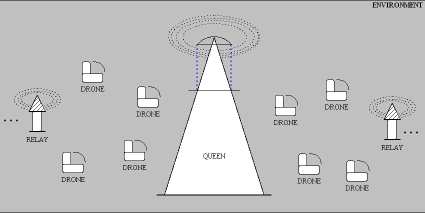
\includegraphics[scale=0.75]{figures/QDTransGen}

\caption{\label{fig:orches}An Orchestrated Robotic Network}

\end{figure}

Such a system should be read analytically rather than heroically. Its
value lies in making allocation, coordination, and dependence visible
enough to measure, perturb, and reproduce.

\textbf{Choice in Runtime.} Choice becomes sharper in an orchestrated system because the meaning
of a decision is not contained within one node alone. A local decision
can change global allocation, system range, energy availability, and
future state formation across the colony. Orchestration therefore
makes it possible to study local and global behavior together.

\textbf{Choice Features.} The relevant features for choice in a distributed system are actionable
alternatives, meaningful constraints, state visibility, and consequences
that propagate beyond the local node. The future engineering task
is to make those features measurable in hardware and software rather
than merely naming them.

\textbf{Choice Quantification.} To quantify choice, the system must exhibit at least two operationally
different pathways under conditions that matter. Those pathways must
be selectable in relation to internal and external state, and their
results must feed back into later behavior. The aim is not to quantify
free will in the metaphysical sense. It is to quantify consequential
selection in a machine architecture.

This is one reason orchestration is so useful. Distributed systems
make it easier to study how one decision influences many later possibilities.
They do not solve the problem automatically, but they widen the experimental
surface on which adaptive behavior can be observed.

\textbf{Why Orchestration Exposes the Limits of AI.} Orchestration makes visible why the older AI categories are too narrow
for this project. A distributed artificial entity is not interesting
primarily because it thinks or acts in a human-like way. It is interesting
because it coordinates, persists, allocates, adapts, and remains
behaviorally coherent under changing conditions. That is the level
at which artificial life becomes experimentally serious.

\section{Embodiment and Experiment}

If the theory is to matter, it must be testable. The method of artificial
systems therefore favors experiments in which abstract claims are
forced into contact with engineering realities. The purpose of this
section is not merely to describe prototypes, but to show how an artificial
entity can be placed under conditions where energy, control, coordination,
and consequence become experimentally visible. In the present state
of the work, one current empirical center is the Volatco board experiment:
an asynchronous multi-node platform where development access, watchdog
control, node communication, power measurement, and reproducible startup
conditions can all be specified in laboratory form.

\textbf{Featured Power.} A featured-power arrangement remains useful here only as a
supporting example of consequential machine behavior. It gives an
artificial system a structured relation to power so that continued
operation depends on successful regulation rather than on constant
external provision. In that narrower sense, energy is not merely a
utility service. It is part of the behavioral problem.

The essential point is simple. Different operational states of the
machine require different levels of available power. If the system
can detect its state, estimate its needs, and request or conserve
power accordingly, then its choices become materially significant.
Failure to regulate well has consequences. Success preserves viability.
That is the part of featured power that still belongs in this manuscript.

\begin{figure}[H]
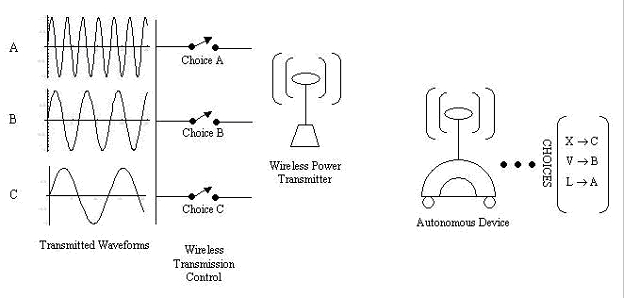
\includegraphics[scale=0.5]{figures/featuredPower}

\caption{Featured Power}

\end{figure}

The sketch represents operational power states that the machine can
request or receive. Level A is full function, Level B is reduced
activity, and Level C is a low-power or sleep condition. The specific
values matter less than the architecture of the choice: the system
is not simply on or off, but capable of moving among energy states
with different behavioral consequences.

At the simplest level, the power relation can still be expressed as:

\begin{equation}
P_{s}=ExI
\end{equation}

What survives from the earlier featured-power work is not a commitment
to a specific transmission scheme, waveform table, or carrier choice.
It is the methodological lesson that power can be made stateful, graded,
and behaviorally consequential. That lesson can now be carried more
cleanly by the Volatco-centered experiments than by preserving a larger
legacy power architecture here.


\textbf{Platforms Under Test.} The design goal is not to bind the method to a single robot body.
The stronger ambition is to develop an experimental pattern that can
be adapted across multiple machine forms. That means distinguishing
between general platform requirements and component-specific tests.
In that spirit there are two broad categories of target:
\begin{enumerate}
\item Generalized platforms,
\item Specific components (hardware and software).
\end{enumerate}

What matters most is that the platform exposes enough state to observe
behavior under consequence. The project does not need to settle large
metaphysical questions in order to be useful. It needs to produce
machines whose regulation, failure, recovery, and adaptation can be
studied without hand-waving.

\textbf{Robotic Software Abstractions.} Software matters here because it is where system state, decision logic,
and behavioral coordination become inspectable. The aim is not software
abstraction for its own sake, but software architecture that makes
adaptation legible and implementable.

\textbf{Software Architecture for Interactive Machines.} The software paradigm proposed here is modular and domain-oriented.
Its purpose is to preserve explicit mappings among sensing, evaluation,
state change, power condition, and action. Whether realized as a domain-specific
language, a layered control stack, or a library architecture, the
important feature is that behavior remains organized around consequential
transitions rather than opaque monolithic execution.

\textbf{Useful Abstractions.} The most useful abstractions are those that report and regulate internal
state: automata-style transitions, monitoring agents, error recovery,
power-state management, and interfaces between sensors and effectors.
These are valuable because they produce scientific data while the
system is operating, degrading, or recovering.

\textbf{Autonomy and Long-Term Behavior.} Autonomy remains central because long-term machine behavior cannot
be studied seriously if every significant correction is supplied by
an operator. The more the system can regulate its own conduct under
constraint, the more meaningful its experimental behavior becomes.

\textbf{The Entropic Circuit.} The entropic circuit is one of the clearest examples of how this manuscript
turns theory into apparatus. Its purpose is to expose the machine
to decline in a controlled form. If the system does not regulate its
power relation successfully, it loses continuity. If it loses continuity,
it loses operational state. This is not life in the full philosophical
sense, but it is a concrete and testable relation between choice,
constraint, and persistence.

That is why the circuit matters. It converts entropy from metaphor
into engineering pressure. It gives the machine something to manage
that affects what it can become next.

\begin{figure}[H]
\centering
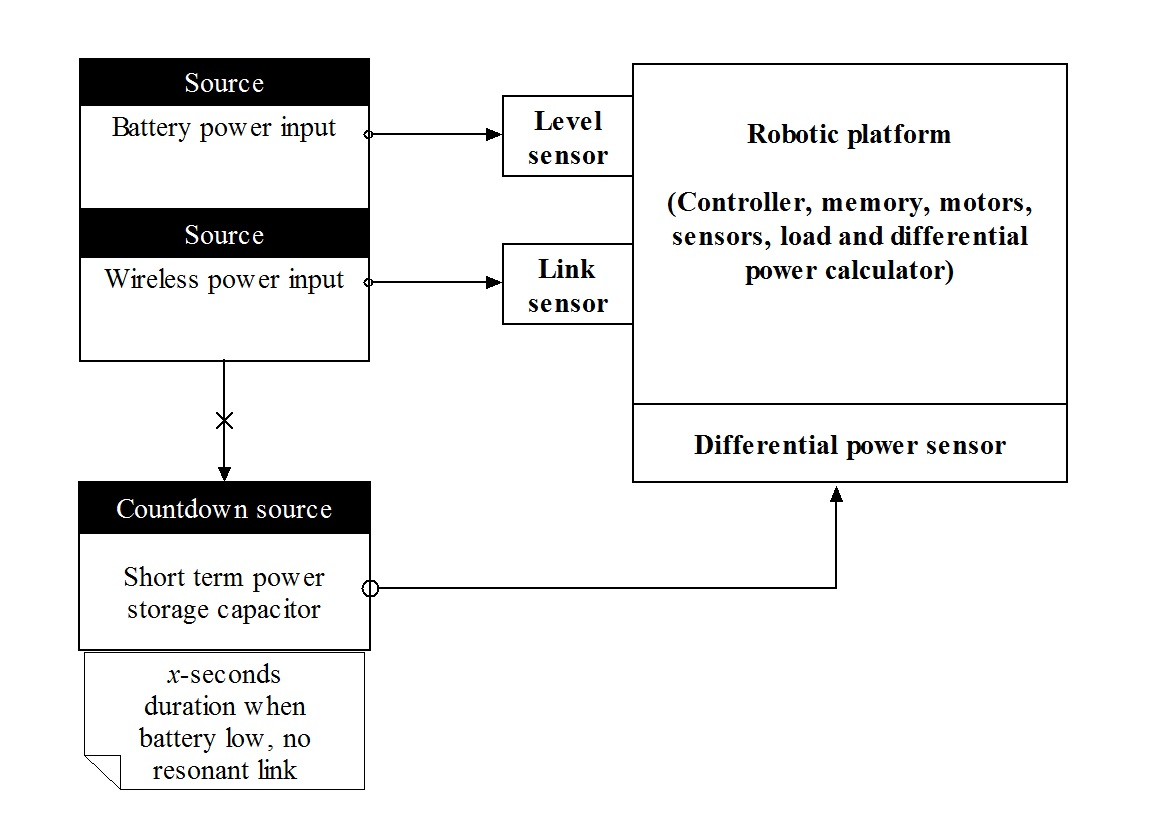
\includegraphics[width=0.9\linewidth]{figures/entropicCircuit}

\caption{The Entropic Circuit}
\end{figure}


\textbf{Scenario Design.} Scenario coding can be understood more simply as the deliberate design
of behavior-rich situations. Instead of treating code as a flat list
of commands, the project treats it as a structured environment in
which sensing, timing, memory, and action can be staged together.
Its future value lies in designing experiments whose behavioral complexity
can scale without dissolving into chaos.

\section{Results and Interpretive Discussion}

The earlier concepts matter only if they can be translated into an
experimental program. The purpose of this section is therefore direct:
to show how the method of artificial systems can be evaluated through
measurable apparatus, software structure, and staged trials. At present,
that evaluation is especially clear when anchored to the Volatco board
as a reproducible substrate rather than to speculative future robot
generalities.

\subsection{Numerical Components of the Theory}

The numerical material in this work matters only when it helps compare
real operating conditions. Geometry, control, electromagnetics, software
structure, and behavioral evaluation enter the manuscript only to
the extent that they produce quantities that can be measured, compared,
and rerun under constraint.

\subsubsection{Experimental Setup}

The setup that matters most in the present manuscript is the Volatco
board environment, because it combines asynchronous node execution
with explicit development and measurement hooks. The methodological
requirements carried forward from earlier measurement work are the following:
\begin{itemize}
\item a stable signal source over the target operating band,
\item impedance measurement for tuned components,
\item spectral analysis for verifying transmitted and received behavior.
\end{itemize}
Calibration remains essential. Measured effects must be attributable
to the system under test rather than to unexamined laboratory artifacts.
The same discipline now applies to the Volatco board: reset mode,
boot mode, watchdog state, serial programming path, pin assignment,
and power-measurement points must all be recorded explicitly so that
an experiment can be rerun by another researcher under substantially
the same conditions.

\subsubsection{Modeling as Secondary Support}

Simulation remains useful, but it is now secondary to the board-level
experiments. Its role is to help narrow search spaces, expose likely
failure regions, and generate testable expectations before hardware
is reworked. It should not be mistaken for the principal evidence
of the manifesto.

The older coupled transmission model is therefore retained only as
a background example of how geometry, receiver posture, and field
behavior can be explored before fabrication. Its continuing value
is heuristic rather than decisive. Even supportive models must be
tied back to explicit material and electrical characteristics if they
are to inform experiment at all.

\subsection{Controllers}

Controllers are where the energetic, perceptual, and behavioral layers
meet. A future artificial-life platform should therefore treat controllers
as explicit objects of design rather than incidental code surrounding
the hardware.

\subsubsection{Visual Robotics and Virtual Controllers}

Virtual controllers matter because they let us prototype choice, orchestration,
and sensor fusion before committing to a specific body. The exact software
stack will change over time, but the principle remains: embodied intelligence
benefits from a simulation layer in which sensing, actuation, timing,
and environmental perturbation can be inspected under controlled conditions.

In such an environment, a robot can be subjected to controlled gravity,
lighting, friction, clutter, and timing conditions while its controllers
are instrumented in detail. The larger point is simple: virtual environments
provide a disciplined route from conceptual manifesto to testable
architecture.

\subsubsection{Agents and their Effectors}

An agent in this document is not a metaphysical claim; it is a software
entity with bounded responsibilities, observable state, and effectors
through which it acts on the rest of the system. Effectors are therefore
the practical bridge between internal evaluation and external consequence.
Treating them explicitly allows the architecture to compare what was
intended, what was executed, and what actually happened in the environment.

\subsection{The Choice Complex}

The Choice Complex is the experimental heart of the manifesto. Its
purpose is to create circumstances under which a machine must regulate
its own continuation under bounded energetic conditions and must do
so through interpretable software and hardware structures. The Featured
Power Environment (FPE) is one such apparatus. It links wireless power,
state monitoring, signaling, and graded operating modes so that the
machine's decisions can be studied as consequential responses rather
than as disembodied classification outputs.
In the current research program, the importance of that apparatus is
not as a finished destination, but as a way of making state, support,
and consequence explicit enough to migrate into a more reproducible
board-level setting.

The immediate experimental objective is to distinguish operating regimes
A, B, and C and their corresponding signaling forms L, V, and X.
The larger point is not the labels themselves, but the requirement
that state, need, and response be made explicit enough to measure.
Future variants may use different signaling schemes, but the essential
idea is stable: the machine must detect its state, communicate its
need, and alter its behavior according to the availability of support.

\subsubsection{The Transmitting Array (Queen)}

The transmitting array names the infrastructure side of the choice
problem. In the legacy apparatus it held the larger energetic reserve,
interpreted requests from the field, and allocated power according
to explicit operating modes. In the current program, the same analytical
role survives in more general form: some part of the system must regulate
support rather than treat it as a constant background condition.

\subsubsection{The Receiving Array (Drone)}

The receiving array names the embodied side of the same problem. It
experiences the field locally, stores or spends received power, and
reports conditions that matter to continued operation. In the Volatco-centered
program, these functions should increasingly migrate toward node-local
state, local signaling, and observable recovery rather than remain
attached to an older receiver architecture.

\subsubsection{The Software Model}

To engage the model, a feedback relationship is established between
stored energy, observed load, and outgoing request signals. A sensor
placed between the storage system and the feed-through line monitors
state in the Entropic Circuit. The controller then transforms that
state into one of three signaling variations, X, V, or L, corresponding
to different operating modes. The details may evolve, but the design
principle is consistent with the method of artificial systems: consequence
must be encoded, transmitted, and acted upon in a way that remains
inspectable.

\subsubsection{The Experiment}

The experiment should be understood as a staged validation program
for the choice methodology rather than a single decisive demonstration.
\begin{itemize}
\item Define a small node set with explicit behavior assignments.
\item Specify boot, reset, watchdog, and communication conditions before
execution.
\item Record power, latency, state transition, and recovery behavior during
the run.
\item Preserve the exact saved program or image used to produce the result.
\item Rerun the same trial under the same stated conditions.
\item Publish discrepancies as well as successes.
\end{itemize}
The duration matters less than the sequence. Each stage should produce
artifacts that can be repeated, criticized, and extended by later
work.

\subsubsection{The Hardware Experiment}

The exact hardware can change across implementations, but three requirements
remain fixed: the source must be stable enough to characterize, the
system under test must be observable enough to debug, and the measurement
chain must be calibrated well enough that relative comparisons are
trustworthy.

Initial trials can be performed at a modest fixed separation, followed
by distance and orientation sweeps. All tests should preserve logs,
photographs, and waveform captures so that the behavioral conclusions
remain tied to physical evidence.

\subsubsection{The Software Experiment}

The software experiment begins with data organization. A machine that
must preserve itself needs a usable memory of power states, requests,
outcomes, timing, and environmental context. A relational database
is one practical way to structure that memory, though the larger point
is architectural rather than vendor-specific: the system must store
enough state to compare present need against prior consequence.

The experiment should therefore evaluate not only whether signals are
transmitted, but whether the software can query, summarize, and act
on their history in time to preserve continued operation. This is
where artificial life becomes more than control theory alone. The
machine is not merely regulating voltage; it is organizing experience
into future behavior.


\subsubsection{Expected Outcomes}

The most useful anticipated conclusion is modest and strong at the
same time: artificial experience can be studied as the accumulation
of bounded consequential selections. A machine that repeatedly interprets
data, organizes it, selects among constrained options, and acts under
penalty will exhibit a pattern of behavior that can be measured and
compared. In functional terms, the flow remains:
\begin{quote}
data \textrightarrow{} information \textrightarrow{} knowledge \textrightarrow{}
decision \textrightarrow{} action
\end{quote}
The significance of this flow is not rhetorical. It gives the manuscript
a concrete engineering target: build systems in which data becomes
usable knowledge quickly enough to alter action before failure occurs.
The machine therefore requires a data management system, a control
layer, and an environment in which better and worse decisions carry
different consequences.

\subsubsection{Further Experiments on Choice and Method}

There are really two coupled experiments to consider: the energetic
infrastructure that makes persistence measurable, and the embodied
behavioral platform on which choice can be studied empirically. In
the current state of the work, the second is best developed on the
Volatco board rather than on a generic classroom robot. The reason
is methodological. The board exposes the exact elements the manifesto
cares about: asynchronous local processes, node-local memory, explicit
communication paths, watchdog-protected persistence, and measurable
power behavior.

That makes the immediate research program more reproducible than a
vague appeal to future robotics. A minimal experiment can define a
signal path, assign behavior to a small set of nodes, specify boot
and reset conditions, state measurable pass/fail criteria, and record
power, latency, and recovery behavior alongside the saved polyForth
program used to produce the result. This is ordinary scientific practice:
the experiment is not merely declared; it is specified so that it
can be rerun.

The simplest meaningful tasks in that environment are correspondingly
modest. One can implement an event-driven sensing loop, a two-node
message handoff, a watchdog recovery routine, or a power audit across
idle and active conditions. Each of these tasks keeps the manifesto
attached to observable architecture. Each asks whether behavior-defined
asynchronous process with in-node memory words can be made explicit,
measurable, and reproducible on the board.

\subsection{Closing Remarks}

The components presented here point toward a concrete research agenda:
\begin{enumerate}
\item New software forms organized around consequence rather than passive
prediction,
\item New hardware forms built to expose energy, state, and dependence,
\item Shared research platforms that connect laboratory robotics, adaptive
control, and artificial life,
\item A clearer path toward machines that are interpretable because their
survival logic is made explicit.
\end{enumerate}
These directions point toward a future research agenda rather than
a final doctrine. If increasingly complex machines are to display
emergent organization, then the most productive next step is not to
argue prematurely about consciousness but to construct systems in
which preservation, depletion, preference, and adaptation can be observed
under controlled tension. Entropy, scarcity, and dependence are therefore
not side issues. They are the very conditions through which richer
synthetic behavior may become legible.

\section{Implications and Conclusion}

The implications of this work are broader than any single transmitter,
robot, or software stack. Its strongest claim is methodological: future
embodied AI systems should be built around explicit dependencies rather
than around the fiction of unlimited compute, unlimited power, or
context-free reasoning.

Even so, the present manifesto is strongest where it stays close to
its current experimental output. That output is not a final universal
robot architecture. It is a reproducible research path in which the
Volatco board serves as one concrete asynchronous substrate for studying
behavior, memory, communication, reset discipline, and power-aware
control under laboratory conditions.

What this manifesto argues, in condensed form, is the following:
\begin{itemize}
\item embodied intelligence should be studied under real energetic and environmental
constraints,
\item orchestration is a first-class architectural principle for artificial
life,
\item choice becomes scientifically useful when it is tied to measurable
consequence,
\item artificial life in this research program is best treated as embodied
AI with behavior-defined asynchronous process and in-node memory words,
\item the proof of that claim is architectural: symbolic organization, behavioral
decomposition, and hybrid substrate execution together establish the
research program,
\item future progress depends on experimental systems that unify hardware,
software, and environment instead of isolating them,
\item the path forward is constructive: build platforms that let these claims
be tested, criticized, and improved.
\end{itemize}

These claims narrow the agenda rather than enlarge it. The next stage
of the work is to refine them through reproducible experiments
that make behavior, state, communication, and energetic dependence
visible under controlled conditions.

\section{Appendix: Volatco Experimental Program}

\subsection{Purpose of the Appendix}

This appendix is reserved for the current experimental substrate of
the manifesto: the Volatco asynchronous computing platform. Its purpose
is not to reopen older speculative roadmaps, replica schemes, or generalized
design inventories. Its purpose is to show, as plainly as possible,
how artificial life is embodied AI and how another researcher could
reproduce or challenge that demonstration in laboratory conditions.

\subsection{Why Volatco Belongs Here}

The main body of this manuscript argues that artificial life in this
research program should be treated as embodied AI with behavior-defined
asynchronous process and in-node memory words. The appendix belongs
to Volatco because the board is one current place where that
claim can be made concrete. It provides many-node execution, node-local
state, explicit communication paths, watchdog supervision, controlled
startup behavior, and inspectable power use in one bounded laboratory
object.

That makes the board more than an implementation convenience. It is
the present demonstration substrate of the manifesto. If the manuscript
is to stand as more than philosophical preference, it must end near
the apparatus through which artificial life is embodied AI can actually
be tested.

\subsection{Experimental Commitments}

The Volatco appendix should be read as a statement of experimental
discipline. Any serious trial on the board should preserve at least
the following:
\begin{enumerate}
\item board identity and revision,
\item node allocation and role assignment,
\item boot mode and reset conditions,
\item watchdog configuration and recovery expectations,
\item pin map and communication path definitions,
\item power source, measurement points, and load conditions,
\item the exact saved polyForth program or image used in the run,
\item pass/fail criteria stated before execution,
\item logs for latency, state transition, recovery, and energy behavior.
\end{enumerate}
These are not procedural niceties. They are the minimum conditions
under which a claim about embodied behavior can become reproducible
rather than anecdotal.

\subsection{Minimal Experiments}

The first experiments need not be grand. They need to be decisive
enough to show whether the architecture carries the behavior the manifesto
assigns to it. A minimal sequence would include:
\begin{enumerate}
\item a single-node event loop with persistent local state,
\item a two-node message handoff with explicit timing and acknowledgement,
\item a watchdog interruption and recovery routine,
\item a power comparison between idle, active, and recovery states,
\item a reset-and-rerun protocol confirming that the same program yields
the same measurable outcome.
\end{enumerate}
Each experiment isolates one architectural obligation while remaining
small enough to debug honestly. Together they test whether asynchronous
local process, node-local memory, and explicit consequence can be
made visible on the board.

\subsection{What Counts as Evidence}

For the purposes of this manifesto, evidence should be ordinary and
inspectable. A valid experimental claim should be accompanied by saved
source, initialization conditions, node assignments, timing records,
power measurements, and a short statement of what changed between
runs. If a behavior appears only once, cannot survive reset, or depends
on undocumented operator intervention, it should not yet be treated
as evidence for artificial life.

This standard is intentionally conservative. Its purpose is to give
the field a repeatable path from conceptual claim to bounded technical
result.

\subsection{Scaling Path}

If the minimal experiments succeed, the next step is not to jump immediately
to anthropomorphic robotics. The next step is to scale the same discipline
across more nodes, richer message structures, stronger recovery behavior,
and tighter power accounting. The research path proceeds by controlled
extension: first local persistence, then multi-node coordination, then
stateful recovery, then larger orchestration problems in which local
choices alter colony-level behavior.

Under that sequence, Volatco does not function as a detour from artificial
life. It functions as the current scientific instrument through which
artificial life can be argued, measured, and revised.

\section*{Epilogue}

The older lineage behind this manifesto deserves explicit acknowledgement
without being turned into review literature. Grey Walter established
an early and durable priority for embodied machine behavior, and Owen
Holland's later recovery of that line helped keep the problem of situated
artificial agency in view. Holland and McFarland also deserve acknowledgement
for giving artificial ethology a clear programmatic form, while Rodney
Brooks helped keep attention on the problem of building materially
embodied, behavior-producing systems across the boundary between artificial
intelligence and artificial life. Ross Ashby remains central for
priority on regulation, stability under disturbance, and adaptive
organization as a state problem.

Several other works mark important boundaries of the design space addressed
here. Abraham Maslow is acknowledged for foregrounding motivation,
growth, and self-actualization as organized features of behavior;
Melissa Bateson, Susan Healy, and T. Andrew Hurly for showing that
choice under constraint can be studied behaviorally; and Giovanni
Stanghellini for treating disembodiment as a serious phenomenological
problem rather than a neutral condition of existence. Isaac Asimov
is acknowledged not as a scientific source but for priority in dramatizing
machine governance and conflict as a public conceptual problem, while
Jean Baudrillard is acknowledged for sharpening questions of simulation
and representation that any manifesto of artificial systems eventually
encounters.

On the constructive side, A. van Deursen is acknowledged for articulating
the trade between domain-specific languages and frameworks; E. F. Codd
for the importance of formal data organization; Stephen Kleene, more
cautiously, for the logical treatment of effective procedure associated
with computable description; and John von Neumann for priority on
self-reproduction as a design problem rather than a mere metaphor.
Andre Kurs, Aristeidis Karalis, Robert Moffatt, J. D. Joannopoulos,
Peter Fisher, and Marin Solja\v{c}i\'{c} are acknowledged for giving
wireless power transfer a modern experimental footing, while Steve
Grand's published work is acknowledged for keeping open the possibility
that artificial life must be grown through situated adaptive process
rather than assembled as static demonstration. The private correspondence
is retained here as part of the project's own historical record rather
than as public literature.

\end{document}
